\section*{Zielsetzung}
In diesem Versuch werden der effektive Dämpfungswiderstand, der Dämpfungswiderstand, bei dem der aperiodische Grenzfall auftritt sowie die Frequenzabhängigkeit gedämpfter und erzwungener Schwingungen bestimmt. Dazu wird ein elektrischer Serienschwingkreis untersucht. 

\section{Theorie}
\label{sec:Theorie}
\subsection{Gedämpfte Schwingung}
In \autoref{fig:rlc} ist die prinzipielle Schaltung eines gedämpften Serienschwingkreises dargestellt. 
\begin{figure}[H]
    \centering
    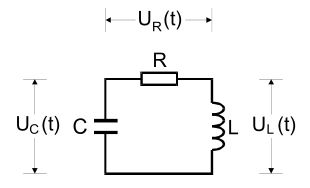
\includegraphics{bilder/rlc.JPG}
    \caption{Schaltung eines gedämpften Serienschwingkreises. \cite{sample}}
    \label{fig:rlc}
  \end{figure}
\noindent
Durch diese Schaltung wird eine gedämpfte Schwingung der Energie realisiert, die zwischen den beiden Speichern (Spule L und Kapazität C) hin und her pendelt. Der Widerstand R sorgt für die Dämpfung der Schwingung, indem er elektrische Energie irreversibel in Wärmeenergie umwandelt. Für diese Schaltung kann mit dem 2. Kirchhoffschen Gesetz eine Differentialgleichung(DGL) ermittelt werden.

\begin{equation}
    U_{\symup{R}} + U_{\symup{C}} + U_{\symup{L}}   = 0     
    \label{eqn:masche}
\end{equation}

\noindent Die Spannungsbeziehungen für die 3 Bauelemente sind durch die Beziehungen
    \begin{align}
        U_{\symup{R}} & = RI \\
        U_{\symup{C}} & = \frac{Q}{C}\\
        U_{\symup{L}} & = L \cdot \symup{\frac{d}{dt}}I 
    \end{align}
\noindent gegeben. 
Mit diesen Beziehungen und $I=\symup{\frac{d}{dt}}Q$ kann die DGL für die Schaltung mit einmaligem Ableiten aufgestellt werden:
\begin{align}
        L  \symup{\frac{d}{dt}}I + RI + \frac{Q}{C} & = 0 \\
       \iff \symup{\frac{d^2}{dt^2}}I + \frac{R}{L} \symup{\frac{d}{dt}}I + \frac{1}{LC}I & = 0 
        \label{eqn:dgl}
\end{align}
    
\noindent Die DGL kann mit einem komplexen $\symup{e}$-Funktionsansatz gelöst werden.
    \begin{equation}
        I(t) = A \cdot \symup{e}^{j \tilde{w} t}
        \label{eqn:dgl2}
    \end{equation}

    \begin{equation}
        \tilde{\omega}_{1,2} = j \frac{R}{2L} \pm \sqrt{\frac{1}{LC}-\frac{R^2}{4L}} 
        \label{eqn:dgl3}
    \end{equation}
    
    \noindent Das heißt $I(t)$ lässt sich durch folgende Gleichung ausdrücken:
    \begin{equation}
        I(t) = A_1 \cdot \symup{e}^{j \tilde{w}_1t} + A_2 \cdot \symup{e}^{j\tilde{w}_2 t} 
    \end{equation}

\noindent Es lassen sich nun 3 unterschiedliche Fälle für die Lösung der DGL, in Abhängigkeit des Wurzelterms in \autoref{eqn:dgl3}, unterscheiden. 
Im ersten Fall ist $\frac{1}{LC} > \frac{R²}{4L²}$ und die Wurzel in \autoref{eqn:dgl3} bleibt reell. Dieser Fall wird als Schwingfall bezeichnet. Der typische Verlauf der Stromstärke für diesen Fall ist in autoref{fig:daempf} dargestellt.
\begin{figure}[H]
    \centering
    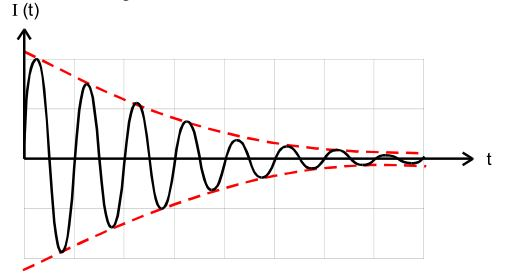
\includegraphics{bilder/daempf.jpg}
    \caption{Qualitativer Verlauf der Stromstärke einer gedämpften Schwingung abhängig von der Zeit. \cite{sample}}
    \label{fig:daempf}
  \end{figure}
\noindent
Die in \autoref{fig:daempf} gestrichelt gezeichnete Einhüllende der Schwingung ist eine e-Funktion der Form
\begin{equation*}
    \pm U_0 e^{-2\pi\mu t} \\ \text{.}
    \label{eqn:einh}
\end{equation*}
\noindent
Für den zweiten Fall gilt:
\begin{equation}
    \frac{1}{LC} < \frac{R^2}{4L^2} 
\end{equation}

\noindent In diesem Fall ist $\tilde{\omega} \in \mathbb{C}$.
Den Fall

\begin{align*}
\frac{1}{LC} &= \frac{R²}{4L²}\\
\iff R &= 2\sqrt{\frac{L}{C}}
\end{align*}

\noindent bezeichnet man als aperiodischen Grenzfall. In diesem Fall bewegt sich $I(t)$ ohne 
Überschwingen am schnellsten gegen 0. 
\subsection{Erzwungene Schwingung}
Um erzwungene Schwingungen mit einem elektrischen Schwingkreis zu realisieren, kann die Schaltung aus \autoref{fig:rlc} zu der Schaltung aus \autoref{fig:erzwungen} erweitert werden. Hier sorgt eine Spannungsquelle mit sinusförmiger Wechselspannung für die äußere Anregung.
\begin{figure}[H]
    \centering
    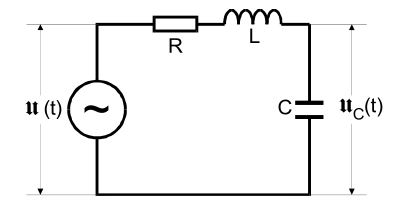
\includegraphics{bilder/erzwungen.JPG}
    \caption{Schaltung zur Erzeugung einer erzwungenen Schwingung mit einem elektrischen Schwingkreis. \cite{sample}}
    \label{fig:erzwungen}
  \end{figure}
\noindent
Die DGL der Schaltung erhält durch diese Veränderung eine Inhomogenität.